% !TEX root = ../../main.tex
\chapter{Wind Mass Loss Rate construction}\label{chap:mass_loss_construction}

\todo{Read N\&L and add detail}

We construct our wind mass loss rates as follows. The total pre-WR mass loss is given by \citet{De_jager:1988}, namely

% \begin{equation}
%     \dot{M}_\text{pre-WR} = \dot{M}_\text{Vink} - \dot{M}_\text{RLF} + \langle \dot{M}_\text{2A}\rangle,\label{eq:pre-wr-ml}
% \end{equation}

\begin{align}
    \log\dot{M}_\text{de Jager} &= -\sum_{n=0}^5 \sum_{\substack{i=0\\j=n-i}}^n a_{ij}\cos\left(i\arccos x_1\right)\cos\left(j\arccos x_2\right),\\
    \dot{M}_\text{pre-WR} &= \sqrt{\frac{Z}{Z_\odot}}10^{\log\dot{M}_\text{de Jager}},\label{eq:pre-wr-ml}
\end{align}

where $x_1 = \frac{\log T-4.05}{0.75}$, $x_2=\frac{\log L-4.6}{2.1}$, and the coefficients $a_{ij}$ are given in Table VI of \citet{De_jager:1988}. We interpolate the bi-stability jump around \SI{25}{\kilo\kelvin} \citep[see, for example,][]{Pauldrach:1990, Vink:1999} with the following regime. Define the constants

\begin{align}
    R_1 &= \left(\frac{Z}{Z_\odot}\right)^{0.13},\label{eq:R1}\\
    R_2 &= -c_1+c_2\log\left(\frac{L}{c_{16}}\right)-c_3\log\left(\frac{M}{c_{15}}\right)-c_4\log\left(1.3R_1\right)+c_5\log\left(\frac{T}{c_{14}}\right)-c_6\left(\log\left[\frac{T}{c_{14}}\right]\right)^2+c_7\log\left(\frac{Z}{Z_\odot}\right),\label{eq:R2} \\
    &\text{and} \notag\\
    R_3 &= -c_8+c_9\log\left(\frac{L}{c_{16}}\right)-c_{10}\log\left(\frac{M}{c_{15}}\right)-c_{11}\log\left(0.65R_1\right)+c_{12}\log\left(\frac{T}{2\times 10^4}\right)+c_{13}\log\left(\frac{Z}{Z_\odot}\right),\label{eq:R3}
\end{align}

where the constants $c_i$ are given in \Cref{tab:bistability_constants}.

\begin{table}[!htbp]
    \centering

    \begin{tabular}{cc|cc|cc|cc}
    \toprule
        Constant & Value & Constant & Value & Constant & Value & Constant & Value \\
    \midrule
        $c_1$ & $6.697$ & $c_5$ & $0.933$ & $c_9$    & $2.210$ & $c_{13}$ & $0.85$  \\
        $c_2$ & $2.194$ & $c_6$ & $10.92$ & $c_{10}$ & $1.339$ & $c_{14}$ & \SI{4e4}{\kelvin} \\
        $c_3$ & $1.313$ & $c_7$ & $0.85$  & $c_{11}$ & $1.601$ & $c_{15}$ & \SI{30}{\msun} \\
        $c_4$ & $1.226$ & $c_8$ & $6.688$ & $c_{12}$ & $1.07$  & $c_{16}$ & \SI[print-unity-mantissa=false]{1e5}{\lsun} \\
    \bottomrule
    \end{tabular}

    \caption[The mass loss rate constants for interpolation around the bi-stability jump.]{The mass loss rate constants for interpolation around the bi-stability jump (\Cref{eq:R1,eq:R2,eq:R3}). This interpolation is shown pictorally in \Cref{fig:bistability}.}
    \label{tab:bistability_constants}
\end{table}

Our mass loss rate becomes:

\begin{equation}
    \dot{M}_\text{BS} = \begin{cases}
        \frac{(T-T_1)10^{R_3}+(T_2-T)\dot{M}_\text{pre-WR}}{2.5\times 10^3} & T_1 < T < T_2 \\
        10^{R_2} & T_2 \leq T \leq T_3 \\
        \frac{(T-T_3)10^{R_2}+(T_4-T)10^{R_3})}{5 \times 10^3} & T_3 < T < T_4 \\
        \frac{(6T_1-T)10^{R_2}+(T-5T_1)\dot{M}_\text{pre-WR}}{10^4} & 5T_1 < T < 6T_1 \\
        \dot{M}_\text{pre-WR} & \text{otherwise}
    \end{cases}
\end{equation}

where $T_1=\SI{10}{\kilo\kelvin}, T_2=\SI{12.5}{\kilo\kelvin}, T_3=\SI{22.5}{\kilo\kelvin}, T_4=\SI{27.5}{\kilo\kelvin}$. This interpolation is shown in \Cref{fig:bistability}. We define

\begin{equation}
    \mathcal{M} = \sqrt{\frac{Z}{Z_\odot}}\times 10^{-13.6 + 1.63\log\left(\frac{L}{L_\odot}\right)+2.22\log X},
\end{equation}

where $X$ is the surface hydrogen abundance of the primary, and then define

\begin{equation}
    \dot{M}_\text{WNL} = \begin{cases}
        5\left(\mathcal{M}-\dot{M}_\text{BS}\right)\left(0.42-X\right)+\dot{M}_\text{BS} & 0.42 > X > 0.4 \\
        \mathcal{M} & \text{otherwise}
    \end{cases}.
\end{equation}

Our total mass loss (provided the star has not depleted its surface helium, which will be discussed below) is now

\begin{equation}
    \dot{M}_\text{A} = \begin{cases}
        10\dot{\mu}\left(\log T-3.9\right) + \dot{M}_\text{BS} & X < 0.42 \text{ and } \log T > 3.9 \\
        \dot{M}_\text{WNL} & X > 0.42 \text{ and } \log T > 4.0 \\
        \dot{M}_\text{BS} & \text{otherwise}
    \end{cases},
\end{equation}

where $\dot{\mu}=\dot{M}_\text{WNL}-\dot{M}_\text{BS}$. Finally, if the surface helium depletes we modify the mass loss rate further, defining

\begin{equation}
    \dot{M}_\text{WC} = \sqrt{\frac{Z}{Z_\odot}}\times 10^{-8.3 + 0.84\log\left(\frac{L}{L_\odot}\right) + 2.04\log X_\text{He} + 1.04\log\left(1-X_\text{He}\right)}
\end{equation}

such that our total mass loss rate becomes (provided $X_\text{H} < 10^{-3}$ and $\log T > 4$)

\begin{equation}
    \dot{M}_\text{B} = \begin{cases}
        100\left(\dot{M}_\text{WC} - \dot{M}_\text{WNL}\right)\left(\mathcal{X}-0.02\right)+\dot{M}_\text{WNL} & \mathcal{X} > 0.02 \\
        \dot{M}_\text{WNL} & \mathcal{X} < 0.02
    \end{cases},
\end{equation}

where $\mathcal{X}=\frac{\frac13 X_\text{C}+\frac14 X_\text{O}}{X_\text{He}}$. The total \citet{Vink:2001} mass-loss rate is then

\begin{equation}
    \dot{M}_\text{wind} = \begin{cases}
        \dot{M}_\text{B} & \text{surface helium depleted} \\
        \dot{M}_\text{A} & \text{otherwise}
    \end{cases}.\label{eq:vink_ml}
\end{equation}

\begin{figure}[!htbp]
    \centering
    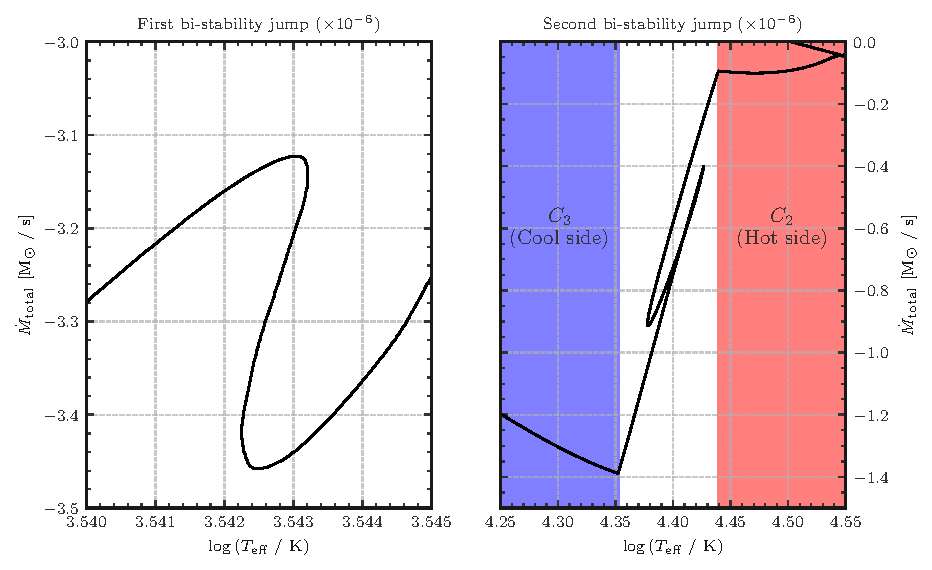
\includegraphics[width=\textwidth]{images/TheorySection/double_bistability_jump.pdf}
    \caption[An illustration of the bi-stability jumps in the mass loss prescription.]{An illustration of the bi-stability jumps in the mass-loss prescription. This illustration was computed for a $\SI{21}{\msun}$ star. \textit{Left plot:} The lower bi-stability jump,  \textit{Right plot:} Shown in blue is the cool side of the bi-stability jump, where $R_3$ (\Cref{eq:R3}) is the interpolation, and shown in red is the hot side, where $R_2$ (\Cref{eq:R2}) is the interpolation.}
    \label{fig:bistability}
\end{figure}
